\section{Реализация}
	
	За постигане на целите на описаната система може да се подходи по различни начини (както и към повечето софтуерни проблеми), но естеството на проблема и незнанието от страна на автора за пълна спецификация на крайния продукт са предпоставки за използване на \ac{AD}.
	
	\ac{AD} е процес, съвкупност от множество практики при разработка на софтуер. Той позволява изучаване на областта, за която се създава продукта, доставя частични работещи версии през определен период от време (най-често на всеки две седмици) и насърчава бързата реакция при настъпване на промени. Терминът е представен от \emph{The Agile Manifesto}\footnote{\url{http://agilemanifesto.org/}} през 2001 г.
	
	\ac{AD} предоставя начини за справяне с проблемите при създаване на софтуерни продукти, но оставя и свобода за персонализиране за съответната среда и разработчици.
	
	\subsection{Процес за реализация на системата}
	
		Предлага се следния персонализиран вариант на \ac{AD} за създаване на системата. Необходимо е извършването на няколко повторения(iterations). За всяко от тях:
	
		\begin{itemize}
			\item Избиране на 2-3 свойства за добавяне към съществуващия продукт от общия списък
			\item За всяко от тях:
				\begin{itemize}
					\item Създават се тестове, които да покажат, че част от свойството работи
					\item Имплементира се логиката необходима за преминаване на тестовете
					\item Кодът се преглежда за начини за промяна с цел улесняване за промяна и по-лесно разбиране
					\item Повтаря се, докато свойството не е напълно имплементирано
				\end{itemize}
			\item Пускат се всички тестове
			\item Преглед и обсъждане на възможности за подобряване на проекта
			\item Текущата версия е готова
		\end{itemize}
		
	\subsection{Повторение I}
	
		За първото повторение от имплементацията на системата се избират най-важните свойства от нея:
		
		\begin{itemize}
			\item Извличане на информация за приложение и запазването й
			\item Регистрация на потребители
			\item Създаване и запазване на препоръки
		\end{itemize}
		
		За извличане на информация за отделните приложения съществуват множество уеб страници, две от които са \url{http://play.google.com/} и \url{http://www.appannie.com/}. Вторият предоставя допълнителна информация, като например ранкът на приложението в различните държави, което може да се окаже предимство при по-задълбочен анализ на всяко приложение.
		
		Създават се тестове, които проверяват дали се взима правилната информация от AppAnnie, като заглавие, описание, категория и т.н. за всяко приложение. Оптимизация, която намаля значително времето за изпълнение на тестовете, е запазване на съдържанието на страницата, която се тества, върху диска на компютъра. Това има един сериозен недостатък - при промяна на страницата, тестовете ще продължат да преминават, тъй като имат стара версия на съдържанието. Този проблем се решава лесно като съдържанието се обновява често ръчно или автоматично.
		
		На фигура ~\ref{figure:spider} е показана клас диаграма на модула \emph{Spider}. Основният клас в него е \emph{AppAnnieSpider}. Той наследява \emph{BaseSpider} от библиотеката \emph{Scrapy} и предоставя основната функционалност за обработка на данните от уеб страницата. Това става чрез задаване на конкретни \emph{XPath}\footnote{\url{http://www.w3.org/TR/xpath/}} изрази. В следващи версии на библиотеката ще е възможно и използването на \emph{CSS}\footnote{\url{http://www.w3.org/TR/CSS2/selector.html}} изрази.
		
		\emph{AppPipeline} отново наследява базов клас от \emph{Scrapy} и неговата цел е да предостави възможност за обработка на обектите, които са извлечени, паралелно. Тук се случва и самото запазване на информацията в базата от данни. \emph{AppItem} има за цел да съхрани информация за приложение.
		
		\begin{figure}[htbp]
			\centering
 			\includegraphics[scale=1.3]{diagrams/spider.1}
			\caption{Клас диаграма на Spider}
			\label{figure:spider}
		\end{figure}
		
		Регистрацията на потребител се състой в събиране и запазване на информация, подадена от клиента. По-ясен поглед върху класа, представляваш потребител, се намира в общия модел на фигура ~\ref{figure:model}
		
		Създаването на добри предложения е това, което показва колко успешна е имплементацията. \ac{CF} предоставя добър подход за решаването на такъв проблем, но оставя голяма част от детайлите да бъдат разгледани от разработчика.
		Това прави писането на тестове още по-важно, защото те позволяват налагане на бързи подобрения, ако бъде намерено ново, по-добро, решение.
		
		\subsubsection{Избор на метрика за сходство}
		
		След събиране на данни за това, какво харесва един потребител, трябва да се разбере колко сходен е той с другите. Това се прави чрез сравняване на всеки двама човека и изчислението на резултат за сходство. За тази цел съществуват няколко подхода. Два от по-известните са: \ac{PC} и \ac{ED}.
		
		\ac{ED} е лесен начин за изчисляване на сходство между двама потребители. Формула \eqref{euclidean-distance} показва процеса за намиране сходността на общи приложения между потребителите \emph{p} и \emph{q}.
		
		\begin{equation}\label{euclidean-distance}
			d(p, q) = \sqrt{\sum\limits_{i=1}^n(q_i - p_i)^2}
		\end{equation}
		
		Така зададена, формулата връща по-високи стойности за оценки, които се различават. Това е неинтуитивно, поради което се заменя връщаща по-високи стойности за приличащи си оценки. Резултатът е в интервала \emph{[0, 1]}\cite{Segaran}. Формула \eqref{euclidean-distance-normalized} показва нормализирана версия на уравнението.

		\begin{equation}\label{euclidean-distance-normalized}
			d(p, q) = \frac{1}{1 + \sqrt{\sum\limits_{i=1}^n(q_i - p_i)^2}}
		\end{equation}
		
		Алгоритъм ~\ref{algorithm:euclidean-distance} е псевдокод за изчисляване на Евклидово сходство. Резултатът от извикване на тази функция е нормализирана стойност в интервала \emph{[0, 1]}.
		
		\vspace{2em}		
		
		\begin{algorithm}[H]
			\label{algorithm:euclidean-distance}
		  \SetKwFunction{Union}{Union}
			\KwData{Two users p and q}
			\KwResult{Euclidean similarity between the users}
			$As \longleftarrow \Union{p.apps, q.apps} $\;
			$res \longleftarrow 0$\;
			\lForEach{app $a$ of the apps $As$}{res += pow(pR[i] - qR[i], 2)}\
			\Return $\frac{1}{1 + res}$\;
			\caption{Евклидово сходство между двама потребители}
		\end{algorithm}
		
		\vspace{2em}
		
		\ac{ED} предоставя лесен и изчислително лек начин за оценка на сходство между два обекта. Методът има един сериозен недостатък - не взима в предвид, когато някои потребители дават високи или ниски оценки за всички приложения(grade inflation\footnote{\url{http://en.wikipedia.org/wiki/Grade_inflation}}).
		
		Описаният проблем се решава от \ac{PC}. Тази метрика е малко по-сложна, защото използва коефициент на сходство. Той показва колко добре две множества от данни може да се поставят на права линия. Формулата е по-сложна, но дава нормализирани резултати. Тя е показана на уравнение ~\eqref{pearson-correlation}
		
		\begin{equation}\label{pearson-correlation}
			r(x, y) = \frac{\sum\nolimits'xy - \frac{\sum\nolimits'x\sum\nolimits'y}{n}}
			{\sqrt{(\sum\nolimits'x^2 - \frac{(\sum\nolimits'x)^2}{n})(\sum\nolimits'y^2 - \frac{(\sum\nolimits'y)^2}{n})}}
		\end{equation}
		
		Алгоритъм ~\ref{algorithm:pearson-correlation} представя псевдокод за изчисление на \ac{PC}.
		
		\vspace{2em}

		\begin{algorithm}[H]
			\label{algorithm:pearson-correlation}
			\SetKwFunction{Length}{Length}
			\SetKwFunction{Sqrt}{Sqrt}
		  \SetKwFunction{SumSquares}{SumSquares}
		  \SetKwFunction{Sum}{Sum}
		  \SetKwFunction{SumProducts}{SumProducts}
			\KwData{Two users p and q}
			\KwResult{Pearson correlation of the users}
			$As \longleftarrow \Union{p.apps, q.apps} $\;
			$n \longleftarrow \Length{As} $\;
			$sum1 \longleftarrow \Sum{As, p} $\;
			$sum2 \longleftarrow \Sum{As, q} $\;
			$sum1Sq \longleftarrow \SumSquares{As, p} $\;
			$sum2Sq \longleftarrow \SumSquares{As, q} $\;
			$sumProd \longleftarrow \SumProducts{As, p, q} $\;
			$num \longleftarrow sumProd - (sum1 * sum2 / n) $\;
			$den \longleftarrow \Sqrt((sum1Sq - sum1^2/n)(sum2Sq - sum2^2/n)) $\;
			\Return $\frac{num}{den}$\;
			\caption{Коефициент на Пиърсън за сходство между двама потребители}
		\end{algorithm}

		\vspace{2em}
		
		\ac{PC} е лоша метрика за свързаност, когато не съществува свързаност \cite{Babenko}. Известен пример за това е показан на фигура ~\ref{figure:anscombe-quartet}. Примерът горе в ляво дава смислена стойност за свързаността между оценките за приложения. В другите графики стойността е същата, но значимостта й не е голяма. Средната стойност и стандартното отклонение са еднакви.
		
		\begin{figure}[htbp]
			\centering	
 			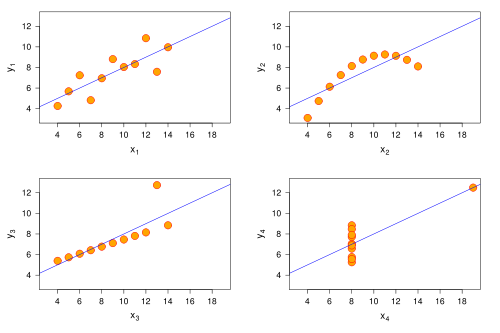
\includegraphics[scale=0.8]{assets/Anscombe-quartet.png}
			\caption{Примери за проблем при използване на свързаност на Пиърсън}
			\label{figure:anscombe-quartet}
		\end{figure}
		
				В система с голям обем данни, вероятността за създаване на подобни проблемни ситуации е много малка. Поради това и сравнително високата ефективност на алгоритъма, той е избран за метрика за сходимост в системата. Имплементацията взима под предвид факта, че може да се наложи неговата замяна. Това прави решението ни лесно за промяна и оставя възможността за набиране на допълнителна информация за проблема.
				
		\subsubsection{Създаване на препоръки}
		
		Алгоритъм ~\ref{algorithm:get-recommendations} създава препоръки за определен потребител. Той е лесен за имплементация, когато има функция, която отговаря на въпроса колко сходни вкусове имат двама потребители. Резултатът от изпълнението му е асоциативен масив подреден в низходящ ред спрямо предположението приложението да се хареса на потребителя. Функцията \emph{Similarity} може да бъде заменена с друга имплементация за сравнение на сходността на двама потребители. Необходимо е тя да предоставя същия интерфейс.
		
		\begin{algorithm}[h]
			\label{algorithm:get-recommendations}
			\SetKwFunction{RelativeComplement}{RelativeComplement}
			\SetKwFunction{Sort}{Sort}
			\SetKwFunction{Reverse}{Reverse}
			\SetKwFunction{Similarity}{Similarity}
			\KwData{All users Us and person p}
			\KwResult{List of recommendations for person p}
			$T \longleftarrow Dict $\;
			$S \longleftarrow Dict $\;
			$A \longleftarrow RelativeComplement(p.ratedApps(), u.ratedApps())$\;
			\For{$ u \in Us$}{
				$sim \longleftarrow Similarity(u, p)$ \;
				\For{$ a \in A$}{
					$T[a] += u.ratingFor(a)* sim$\;
					$S[a] += sim$\;				
				}
			}
			\For{$ t, a \in T$}{
				$R[t/S[app]] = app$ \;
			}
			$Sort(R)$\;
			$Reverse(R)$\;
			\Return $R$\;
			\caption{Създаване на препоръки за потребител}
		\end{algorithm}
		
		Запазването на предложения е лесно, благодарение на общия модел на системата. Тази задача се изпълнява от друг модул на системата.
		
		\subsection{Повторение II}
		
		Благодарение на изпълнението на предишното повторение, системата придобива по-ясен вид и доставя най-необходимата функционалност. Във второто повторение се обръща внимание и на клиента. Имплементацията включва:
		
		\begin{itemize}
			\item Предоставяне на препоръки от сървъра
			\item Вземане на препоръки от сървъра
			\item Изпращане информация за потребителя на сървъра
			\item Приемане на информация за потребителя
		\end{itemize}
		
		Тези свойства се групират две по две и по този начин се разработват паралелно. Това е незадължително при разработка, използваща създаване на тестове преди самата имплементация. Те имитират ролята на сървър, както и тази на клиент, при провеждане на изпълнение.
		
		За даване на препоръки, сървърът предоставя \ac{API}, като използва \emph{REST} протокол и кодира данните в \emph{JSON} формат. Тази архитектура се изгражда на отворени и безплатни стандарти, които модерните уеб технологии предоставят. Липсата на единен стандарт, който задължително трябва да се спазва, за да може едно \ac{API} да бъде наречено \emph{REST-пълно}, води до неясен подход за създаване на добра имплементация.
		
		Някои чести проблеми при създаване на подобна архитектура са\cite{Vitvar}
		
		\begin{itemize}
			\item Използване на \emph{GET} за всички видове заявки
			\item Неспазване на кодовете за отговор
			\item Неспазване правилата за кеширане
		\end{itemize}
		
		\emph{Bottle} предоставя лесен и скалируем начин за справяне с тези и други проблеми, като някои от решенията се взимат автоматично от библиотеката.
		